\chapter{Une alimentation équilibrée}\label{ch:g3:balanced-diet}

Un chantier a besoin de briques, de ciment, de planches --- et de
carburant pour les machines. Ton corps est un chantier qui ne ferme
jamais~: il grandit, se répare et court partout toute la journée.
Ses livraisons arrivent trois ou quatre fois par jour, dans une
assiette. Que doivent-elles contenir~? C'est la question de
l'alimentation.

\section{Pourquoi le corps a besoin de nourriture}

\begin{proposition}[Les deux rôles de la nourriture]\label{prop:g3:balanced-diet:jobs}
La nourriture joue deux rôles différents~:
\begin{enumerate}
  \item elle fournit de l'\emph{énergie}\index{énergie (des
        aliments)} --- de quoi bouger, se tenir au chaud, faire
        tourner le cœur et le cerveau, même pendant le \omterm{prop:g1:healthy-habits:needs}{sommeil}~;
  \item elle fournit du \emph{matériau de construction} --- ce que
        le corps utilise pour grandir, fabriquer du \omterm{def:g3:bones-and-muscles:muscle}{muscle} et de
        l'\omterm{def:g3:bones-and-muscles:skeleton}{os}, réparer les éraflures et remplacer les parties usées.
\end{enumerate}
Une alimentation doit livrer les deux, chaque jour.
\end{proposition}
\admitted

\begin{example}[Du carburant même au repos]\label{ex:g3:balanced-diet:rest}
Même allongé parfaitement immobile, tu dépenses de l'\omterm{prop:g3:balanced-diet:jobs}{énergie}~: le
cœur bat, la poitrine se soulève et s'abaisse, le corps reste chaud
à environ $\qty{37}{\degreeCelsius}$ quel que soit le temps. Cet
abonnement permanent explique pourquoi sauter un repas rend faible
et frileux, et pas seulement affamé.
\end{example}

\section{Les familles d'aliments}

\begin{definition}[Les familles d'aliments]\label{def:g3:balanced-diet:families}
On range les aliments en \emph{familles d'aliments}\index{famille
d'aliments} selon ce qu'ils apportent~:
\begin{itemize}
  \item \emph{\omterm{prop:g3:flowers-fruits-seeds:transform}{fruits} et légumes} --- vitamines, fibres et eau~; la
        famille de la fraîcheur~;
  \item \emph{céréales et féculents} (pain, pâtes, riz, pommes de
        terre) --- la famille de l'\omterm{prop:g3:balanced-diet:jobs}{énergie} qui dure~;
  \item \emph{produits laitiers} (\omterm{def:g2:animals-grow-up:born}{lait}, yaourt, fromage) --- la
        famille qui construit les \omterm{def:g3:bones-and-muscles:skeleton}{os}~;
  \item \emph{viande, poisson et \omterm{def:g2:animals-grow-up:born}{œufs}} --- la famille qui construit
        le corps~;
  \item \emph{matières grasses} (beurre, huile) --- de l'\omterm{prop:g3:balanced-diet:jobs}{énergie}
        concentrée, nécessaire en petites quantités~;
  \item \emph{produits sucrés} --- un plaisir rapide, nécessaire
        pas du tout~: la famille des douceurs~;
  \item et l'\emph{eau}\index{eau (boisson)} --- la seule boisson
        dont le corps ait besoin, tout au long de la journée.
\end{itemize}
\end{definition}

\begin{omfigure}
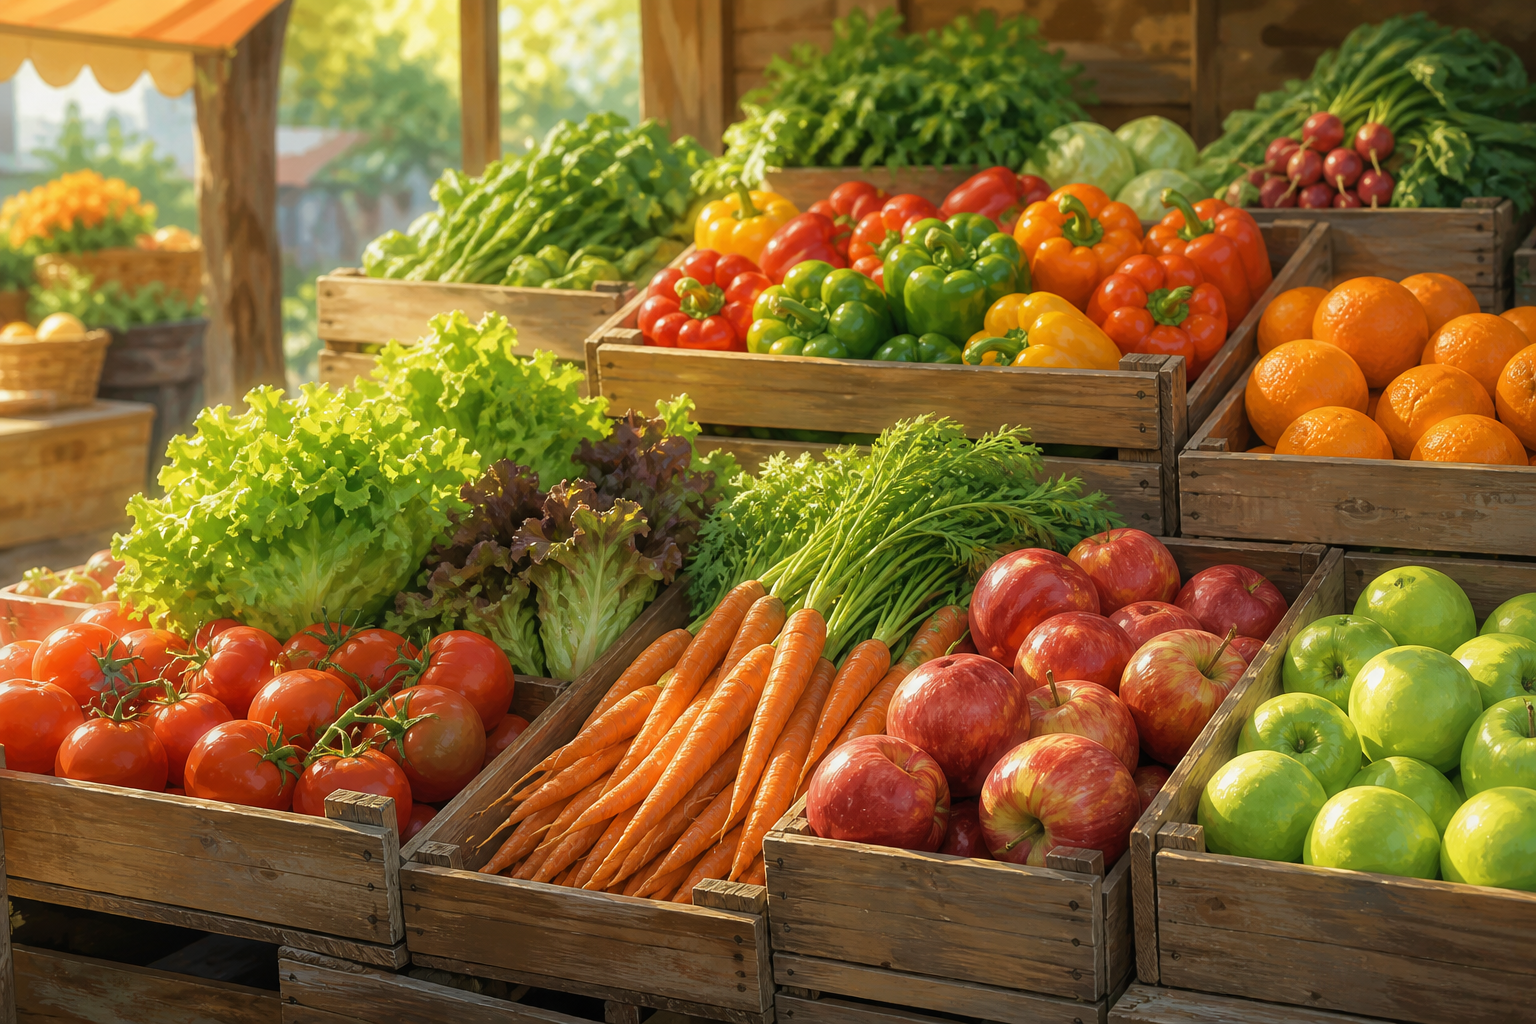
\includegraphics[width=0.62\linewidth]{images/book1/ai/g3-diet-market.png}

{\small La famille de la fraîcheur au marché~: le coin de l'assiette
le plus souvent oublié, ici en aucun danger de l'être.}
\end{omfigure}

\begin{omfigure}
\begin{tikzpicture}
  % plate
  \draw[thick] (0,0) circle (2.8);
  % half: vegetables/fruit
  \draw[thick, fill=omMeth!14] (0,0) -- (0,2.8)
    arc[start angle=90, end angle=270, radius=2.8] -- cycle;
  % quarter: starchy
  \draw[thick, fill=omProp!14] (0,0) -- (0,-2.8)
    arc[start angle=270, end angle=340, radius=2.8] -- cycle;
  % quarter: builders
  \draw[thick, fill=omThm!12] (0,0) -- ({2.8*cos(340)},{2.8*sin(340)})
    arc[start angle=-20, end angle=90, radius=2.8] -- cycle;
  \node[font=\small, align=center] at (-1.4,0.2)
    {fruits et\\ légumes\\ (la moitié de l'assiette)};
  \node[font=\small, align=center] at (1.0,-1.45)
    {pain,\\ pâtes, riz};
  \node[font=\small, align=center] at (1.3,1.0)
    {viande, poisson,\\ œuf ou laitage};
  % water glass
  \draw[thick] (4.0,-0.5) -- (4.1,1.0) -- (5.0,1.0) -- (5.1,-0.5)
    -- cycle;
  \fill[omDef!25] (4.04,-0.44) -- (4.12,0.75) -- (4.98,0.75)
    -- (5.06,-0.44) -- cycle;
  \node[font=\small, align=center] at (4.55,-1.0) {eau};
\end{tikzpicture}

{\small Une assiette bien équilibrée~: moitié fraîcheur, un quart
d'\omterm{prop:g3:balanced-diet:jobs}{énergie} qui dure, un quart de bâtisseurs --- et de l'eau dans le
verre.}
\end{omfigure}

\begin{example}[Équilibrer un déjeuner]\label{ex:g3:balanced-diet:lunch}
Des pâtes à la sauce tomate, un morceau de poisson, des haricots
verts, un yaourt, une pomme, de l'eau~: toutes les familles
présentes, les douceurs absentes --- un déjeuner équilibré. Des
frites, un soda et une barre chocolatée nourrissent exactement deux
familles (matières grasses et sucre) et sautent celles que le
chantier attendait.
\end{example}

\begin{remark}[Pas d'aliments interdits, seulement des oubliés]\label{rem:g3:balanced-diet:balance}
L'équilibre se mesure sur des jours, pas sur des bouchées. Une part
de gâteau d'anniversaire ne casse aucune règle --- l'ennui n'est
jamais une douceur, ce sont les douceurs \emph{à la place} des
familles, jour après jour. La question utile à chaque repas n'est
pas «~cet aliment est-il mauvais~?~» mais «~quelle famille ai-je
oubliée aujourd'hui~?~».
\end{remark}

\section{Adapter la nourriture à la journée}

\begin{proposition}[Les besoins changent avec la journée et la personne]\label{prop:g3:balanced-diet:needs}
La quantité d'\omterm{prop:g3:balanced-diet:jobs}{énergie} dont un corps a besoin dépend de qui il est et
de ce qu'il fait~: un enfant qui grandit a proportionnellement
besoin de plus de matériau de construction qu'un adulte~; une
journée de sport ou de froid brûle plus d'\omterm{prop:g3:balanced-diet:jobs}{énergie} qu'un après-midi
de lecture. La faim grandit avec la dépense du corps.
\end{proposition}
\admitted

\begin{example}[Pourquoi le petit déjeuner compte]\label{ex:g3:balanced-diet:breakfast}
Au matin, le corps a tourné toute la nuit --- cœur, souffle, chaleur
--- sans la moindre livraison. Le petit déjeuner le réapprovisionne
pour les leçons de la matinée et les courses dans la cour. Saute-le,
et vers le milieu de la matinée le chantier manque~: ventre qui
gargouille, attention qui s'échappe, aucune force pour jouer.
\end{example}

\begin{method}[Vérifier l'équilibre d'une journée]\label{met:g3:balanced-diet:check}
En fin de journée, passe la liste en revue~:
\begin{enumerate}
  \item des \omterm{prop:g3:flowers-fruits-seeds:transform}{fruits} ou des légumes à chaque repas~? (objectif~:
        environ cinq portions dans la journée)
  \item un féculent à chaque repas pour l'\omterm{prop:g3:balanced-diet:jobs}{énergie} qui dure~?
  \item les bâtisseurs présents --- des laitages plusieurs fois, et
        de la viande, du poisson ou des \omterm{def:g2:animals-grow-up:born}{œufs} une ou deux fois~?
  \item de l'eau comme boisson de la journée~?
  \item les douceurs~: en petite quantité, pas en plat principal~?
\end{enumerate}
Quelle que soit la famille qui manque, invite-la demain.
\end{method}

\section{Exercices}

\begin{exercise}[$\star$]\label{exo:g3:balanced-diet:1}
Quels sont les deux rôles de la nourriture~? Donne une \omterm{def:g3:balanced-diet:families}{famille
d'aliments} qui sert surtout chacun d'eux.
\end{exercise}

\begin{exercise}[$\star$]\label{exo:g3:balanced-diet:2}
Nomme les \omterm{def:g3:balanced-diet:families}{familles d'aliments}, et la seule boisson dont le corps ait
besoin.
\end{exercise}

\begin{exercise}[$\star$]\label{exo:g3:balanced-diet:3}
Range ces courses par familles~: riz, yaourt, carottes, \omterm{def:g2:animals-grow-up:born}{œufs},
beurre, pommes, pain.
\end{exercise}

\begin{exercise}[$\star$]\label{exo:g3:balanced-diet:4}
Pourquoi le corps dépense-t-il de l'\omterm{prop:g3:balanced-diet:jobs}{énergie} même pendant le
\omterm{prop:g1:healthy-habits:needs}{sommeil}~? Nomme deux dépenses de la nuit.
\end{exercise}

\begin{exercise}[$\star$]\label{exo:g3:balanced-diet:5}
Vérifie le déjeuner «~pâtes, poisson, haricots verts, yaourt, pomme,
eau~» avec l'assiette équilibrée de la figure~: à quelle partie de
l'assiette appartient chaque aliment~?
\end{exercise}

\begin{exercise}[$\star$]\label{exo:g3:balanced-diet:6}
Pourquoi le petit déjeuner est-il particulièrement important~? Que
se passe-t-il au milieu de la matinée sans lui~?
\end{exercise}

\begin{exercise}[$\star$]\label{exo:g3:balanced-diet:7}
Qui a proportionnellement besoin de plus de matériau de
construction~: un enfant ou un adulte~? Pourquoi~?
\end{exercise}

\begin{exercise}[$\star$]\label{exo:g3:balanced-diet:8}
À toi d'essayer~: applique \cref{met:g3:balanced-diet:check} à ta
propre journée, honnêtement. Quelle famille as-tu oubliée --- et
laquelle est apparue plus que sa part~?
\end{exercise}

\begin{exercise}[$\star\star$]\label{exo:g3:balanced-diet:9}
«~Les bonbons sont interdits~!~» Est-ce ce que dit ce chapitre~?
Donne la règle plus précise de \cref{rem:g3:balanced-diet:balance}.
\end{exercise}

\begin{exercise}[$\star\star$]\label{exo:g3:balanced-diet:10}
Pendant des vacances au ski, tout le monde a plus faim qu'à la
maison. Explique avec \cref{prop:g3:balanced-diet:needs} --- nomme
les deux dépenses supplémentaires qu'ajoute une journée froide et
sportive.
\end{exercise}
